\documentclass{article}

% content/resources/templates/preamble.tex
\usepackage[margin=0.6in]{geometry}
\author{Milav Dabgar}
\usepackage{amsmath,amssymb,amsthm}
\usepackage{booktabs}
\usepackage{multirow}
\usepackage{xcolor}
\usepackage{tcolorbox}
\tcbuselibrary{breakable,skins}
\usepackage[colorlinks=true,linkcolor=blue]{hyperref}
\usepackage{titlesec}
\usepackage{enumitem}
\usepackage{tikz}
\usepackage{pgfplots}
\usepackage{circuitikz}
\usepackage[version=4]{mhchem}
\usepackage{longtable}
\usepackage{array}
\usepackage{float}
\usepackage{caption}
\usepackage{listings}

\lstset{
  basicstyle=\small\ttfamily,
  breaklines=true,
  breakatwhitespace=false,
  postbreak=\mbox{\textcolor{red}{$\hookrightarrow$}\space},
  float=false,
  numbers=left,
  numberstyle=\tiny\color{gray},
  numbersep=10pt,
  xleftmargin=2em,
  keywordstyle=\color{blue},
  commentstyle=\color{green!60!black},
  stringstyle=\color{purple},
  backgroundcolor=\color{gray!5},
  showstringspaces=false,
  tabsize=2,
  captionpos=b,
  keepspaces=true,
  columns=flexible
}

\pgfplotsset{compat=1.18}
\usetikzlibrary{shapes,arrows,positioning,calc,patterns,decorations.pathmorphing,decorations.markings,arrows.meta}

% Color scheme
\definecolor{headcolor}{RGB}{0,102,204}
\definecolor{keycolor}{RGB}{220,20,60}
\definecolor{solutioncolor}{RGB}{34,139,34}
\definecolor{mnemoniccolor}{RGB}{148,0,211}
\definecolor{codecolor}{RGB}{0,0,100}

% Spacing
\setlength{\parskip}{3pt}
\setlist[itemize]{nosep}
\setlist[enumerate]{nosep}

% Title formatting
\titleformat{\section}{\Large\bfseries\color{headcolor}}{\thesection}{1em}{}
\titleformat{\subsection}{\large\bfseries\color{headcolor}}{\thesubsection}{1em}{}

% Pandoc tightlist compatibility
\providecommand{\tightlist}{%
  \setlength{\itemsep}{0pt}\setlength{\parskip}{0pt}}

% Pandoc longtable compatibility
\newcounter{none}
\def\thenone{}


% content/resources/templates/english-boxes.tex

% Custom environments
\newtcolorbox{solutionbox}{
 breakable,
 enhanced,
 colback=solutioncolor!5!white,
 colframe=solutioncolor!75!black,
 fonttitle=\bfseries,
 title=Solution
}

\newtcolorbox{solutionboxnobreak}{
 colback=solutioncolor!5!white,
 colframe=solutioncolor!75!black,
 fonttitle=\bfseries,
 title=Solution
}

\newtcolorbox{keyformula}{
 breakable,
 enhanced,
 colback=keycolor!5!white,
 colframe=keycolor!75!black,
 fonttitle=\bfseries,
 title=Key Formula
}

\newtcolorbox{mnemonicboxenv}{
 breakable,
 enhanced,
 colback=mnemoniccolor!5!white,
 colframe=mnemoniccolor!75!black,
 fonttitle=\bfseries,
 title=Mnemonic
}

\newcommand{\mnemonicbox}[1]{%
  \begin{mnemonicboxenv}
    #1
  \end{mnemonicboxenv}
}


% Custom commands for GTU solutions
% This file defines semantic commands for consistent formatting

% Question command with automatic formatting
\newcommand{\question}[2]{%
  \section*{Question #1}%
  \textbf{#2}%
}

% OR question variant
\newcommand{\questionor}[2]{%
  \section*{Question #1 OR}%
  \textbf{#2}%
}

% Proper table environment with caption
\newenvironment{answertable}[1]{%
  \begin{table}[htbp]
  \centering
  \caption{#1}
}{%
  \end{table}
}

% Proper figure environment for diagrams
\newenvironment{answerdiagram}[1]{%
  \begin{figure}[htbp]
  \centering
  \caption{#1}
}{%
  \end{figure}
}

% Semantic markup for key terms
\newcommand{\keyword}[1]{\textbf{#1}}
\newcommand{\code}[1]{\texttt{#1}}
\newcommand{\classname}[1]{\texttt{#1}}
\newcommand{\methodname}[1]{\texttt{#1}}

% Proper quotation marks
\newcommand{\mnemonic}[1]{``#1''}


\title{Elements of Electrical \& Electronics Engineering (1313202) - Winter 2024 Solution}
\date{January 17, 2024}

\begin{document}
\maketitle

\questionmarks{1(a)}{3}{Explain difference between Active and passive network.}

\begin{solutionbox}
\begin{tabulary}{\linewidth}{|L|L|}
\hline
\textbf{Active Network} & \textbf{Passive Network} \\ \hline
Contains at least one active element (voltage/current source) & Contains only passive elements (R, L, C) \\ \hline
Can deliver energy to the circuit & Cannot deliver energy to the circuit \\ \hline
Can amplify signal power & Cannot amplify signal power \\ \hline
\end{tabulary}
\end{solutionbox}

\begin{mnemonicbox}
\mnemonic{Active Adds Power, Passive Parts Take}
\end{mnemonicbox}

\questionmarks{1(b)}{4}{State and explain Kirchhoff's voltage law (KVL).}

\begin{solutionbox}
\textbf{Statement:} Kirchhoff's Voltage Law (KVL) states that the algebraic sum of all voltages around any closed loop in a circuit is zero.

\textbf{Mathematically:} $V_1 + V_2 + V_3 + V_4 = 0$ or $\sum V = 0$

\begin{center}
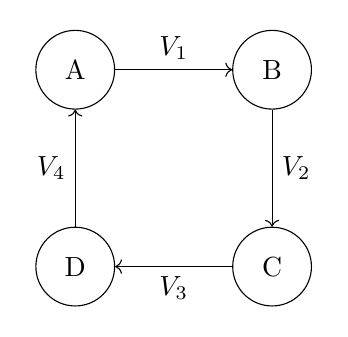
\begin{tikzpicture}[
    node distance=2.5cm,
    state/.style={circle, draw, minimum size=1cm}
]
    \node[state] (A) {A};
    \node[state] (B) [right of=A] {B};
    \node[state] (D) [below of=A] {D};
    \node[state] (C) [below of=B] {C};

    \draw[->] (A) -- node[above] {$V_1$} (B);
    \draw[->] (B) -- node[right] {$V_2$} (C);
    \draw[->] (C) -- node[below] {$V_3$} (D);
    \draw[->] (D) -- node[left] {$V_4$} (A);
\end{tikzpicture}
\end{center}

\textbf{Sign Convention:}
\begin{itemize}
    \item \textbf{Voltage Drop}: When passing through a resistor in direction of current, voltage is negative.
    \item \textbf{Voltage Rise}: When passing through a source from negative to positive, voltage is positive.
\end{itemize}
\end{solutionbox}

\begin{mnemonicbox}
\mnemonic{Voltage Loop Equals Zero}
\end{mnemonicbox}

\questionmarks{1(c)}{7}{Define the following terms: (1) Charge (2) Current (3) Potential (4) E.M.F. (5) Inductance (6) Capacitance (7) Frequency.}

\begin{solutionbox}
\begin{tabulary}{\linewidth}{|L|L|}
\hline
\textbf{Term} & \textbf{Definition} \\ \hline
\textbf{Charge} & The quantity of electricity measured in coulombs (C). \\ \hline
\textbf{Current} & The rate of flow of electric charge measured in amperes (A). \\ \hline
\textbf{Potential} & The electrical pressure or energy per unit charge measured in volts (V). \\ \hline
\textbf{E.M.F.} & Electromotive Force is the energy supplied by a source per unit charge measured in volts (V). \\ \hline
\textbf{Inductance} & The property of an electric circuit that opposes change in current, measured in henries (H). \\ \hline
\textbf{Capacitance} & The ability of a body to store electrical charge, measured in farads (F). \\ \hline
\textbf{Frequency} & Number of complete cycles per second, measured in hertz (Hz). \\ \hline
\end{tabulary}
\end{solutionbox}

\begin{mnemonicbox}
\mnemonic{Coulombs' Flow Pressurized by Energy Induces Capacitive Fluctuations}
\end{mnemonicbox}

\questionmarks{1(c) OR}{7}{State Ohm's law. Write its application and limitation.}

\begin{solutionbox}
\textbf{Statement:} Ohm's Law states that the current flowing through a conductor is directly proportional to the potential difference and inversely proportional to the resistance, provided physical conditions (temperature) remain constant.

\textbf{Formula:} $V = I \times R$
\begin{center}
\begin{circuitikz}
    \draw (0,0) to[battery1, l=$V$] (0,2) -- (2,2) to[R, l=$R$, i=$I$] (2,0) -- (0,0);
\end{circuitikz}
\end{center}

Where: $V$ = Voltage (V), $I$ = Current (A), $R$ = Resistance ($\Omega$).

\textbf{Applications:}
\begin{itemize}
    \item Circuit design and analysis.
    \item Power consumption calculations.
    \item Component value determination.
    \item Voltage divider networks.
    \item Current divider networks.
\end{itemize}

\textbf{Limitations:}
\begin{itemize}
    \item Valid only for linear components.
    \item Not applicable to non-ohmic devices (diodes, transistors).
    \item Invalid at high temperatures.
    \item Not valid for semiconductors.
    \item Cannot be applied to non-linear resistive elements.
\end{itemize}
\end{solutionbox}

\begin{mnemonicbox}
\mnemonic{Volts Reveal Amps' Motion}
\end{mnemonicbox}

\questionmarks{2(a)}{3}{Draw and explain energy band diagrams for insulator, conductor and Semiconductor.}

\begin{solutionbox}
\begin{center}
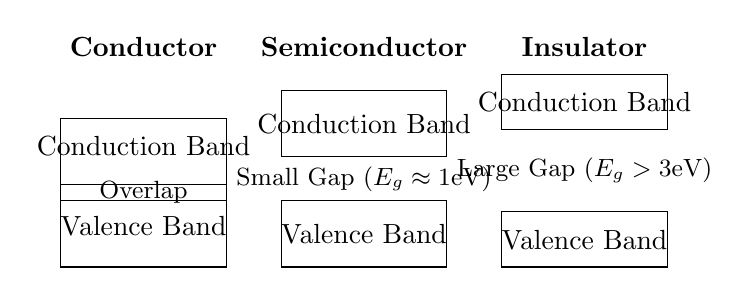
\begin{tikzpicture}[scale=0.7]
    % Conductor
    \node at (1.5,4) {\textbf{Conductor}};
    \draw (0,0) rectangle (3,1.5); \node at (1.5,0.75) {Valence Band};
    \draw (0,1.2) rectangle (3,2.7); \node at (1.5,2.2) {Conduction Band};
    \node at (1.5,1.35) {\small Overlap};

    % Semiconductor
    \node at (5.5,4) {\textbf{Semiconductor}};
    \draw (4,0) rectangle (7,1.2); \node at (5.5,0.6) {Valence Band};
    \draw (4,2.0) rectangle (7,3.2); \node at (5.5,2.6) {Conduction Band};
    \node at (5.5,1.6) {\small Small Gap ($E_g \approx 1$eV)};

    % Insulator
    \node at (9.5,4) {\textbf{Insulator}};
    \draw (8,0) rectangle (11,1.0); \node at (9.5,0.5) {Valence Band};
    \draw (8,2.5) rectangle (11,3.5); \node at (9.5,3.0) {Conduction Band};
    \node at (9.5,1.75) {\small Large Gap ($E_g > 3$eV)};
\end{tikzpicture}
\end{center}

\begin{itemize}
    \item \textbf{Conductor}: Valence and conduction bands overlap, allowing free electron movement.
    \item \textbf{Semiconductor}: Small energy gap (0.7-3 eV) between bands allows limited conduction.
    \item \textbf{Insulator}: Large energy gap ($>3$ eV) prevents electrons from moving to conduction band.
\end{itemize}
\end{solutionbox}

\begin{mnemonicbox}
\mnemonic{Conductors Overlap, Semiconductors Jump Small, Insulators Block All}
\end{mnemonicbox}

\questionmarks{2(b)}{4}{Write statement of Maximum power transfer theorem and reciprocity theorem.}

\begin{solutionbox}
\begin{tabulary}{\linewidth}{|L|L|}
\hline
\textbf{Theorem} & \textbf{Statement} \\ \hline
\textbf{Maximum Power Transfer Theorem} & Maximum power is transferred from source to load when the load resistance equals the source internal resistance ($R_L = R_S$). \\ \hline
\textbf{Reciprocity Theorem} & In a linear, bilateral network, if voltage source $E$ in branch 1 produces current $I$ in branch 2, then the same voltage source $E$ in branch 2 will produce the same current $I$ in branch 1. \\ \hline
\end{tabulary}
\end{solutionbox}

\begin{mnemonicbox}
\mnemonic{Match Resistance for Maximum Power; Swap Sources, Current Stays}
\end{mnemonicbox}

\questionmarks{2(c)}{7}{Explain the formation and conduction of N-type materials.}

\begin{solutionbox}
\textbf{Formation Process:}
\begin{itemize}
    \item Pure silicon/germanium doped with pentavalent impurity atoms (P, As, Sb).
    \item Impurity atoms have 5 valence electrons (silicon has 4).
    \item Four electrons form covalent bonds, fifth becomes free electron.
    \item Creates excess negative charge carriers.
\end{itemize}

\begin{center}
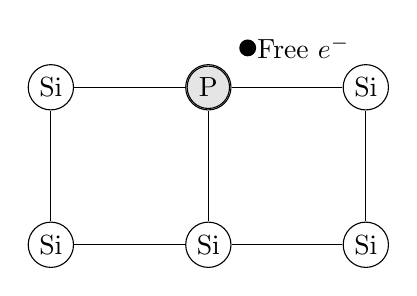
\begin{tikzpicture}
    % Silicon lattice
    \foreach \x in {0,2,4}
        \foreach \y in {0,2}
            \node[circle, draw, inner sep=2pt] at (\x,\y) {Si};
    
    % Impurity
    \node[circle, draw, fill=gray!20, inner sep=2pt] at (2,2) {P};
    
    % Bonds
    \draw (0.3,0) -- (1.7,0); \draw (2.3,0) -- (3.7,0);
    \draw (0.3,2) -- (1.7,2); \draw (2.3,2) -- (3.7,2);
    \draw (0,0.3) -- (0,1.7); \draw (2,0.3) -- (2,1.7); \draw (4,0.3) -- (4,1.7);
    
    % Free electron
    \draw[fill=black] (2.5,2.5) circle (0.1) node[right] {Free $e^-$};
\end{tikzpicture}
\end{center}

\textbf{Conduction Mechanism:}
\begin{itemize}
    \item \textbf{Majority Carriers}: Electrons.
    \item \textbf{Minority Carriers}: Holes.
    \item Electron movement provides electrical conduction.
    \item Even at room temperature, free electrons enable current flow.
\end{itemize}
\end{solutionbox}

\begin{mnemonicbox}
\mnemonic{Pentavalent Provides Plus-One Electron}
\end{mnemonicbox}

\questionmarks{2(a) OR}{3}{Define valence band, conduction band and forbidden gap.}

\begin{solutionbox}
\begin{tabulary}{\linewidth}{|L|L|}
\hline
\textbf{Term} & \textbf{Definition} \\ \hline
\textbf{Valence Band} & Energy band occupied by valence electrons that are bound to specific atoms in the solid. \\ \hline
\textbf{Conduction Band} & Higher energy band where electrons can move freely throughout the material, enabling electrical conduction. \\ \hline
\textbf{Forbidden Gap} & Energy region between valence and conduction bands where no electron states exist. \\ \hline
\end{tabulary}
\end{solutionbox}

\begin{mnemonicbox}
\mnemonic{Valence Binds, Conduction Flows, Forbidden Gaps Block}
\end{mnemonicbox}

\questionmarks{2(b) OR}{4}{Define the terms active power, reactive power and power factor with power triangle.}

\begin{solutionbox}
\textbf{Power Triangle:}
\begin{center}
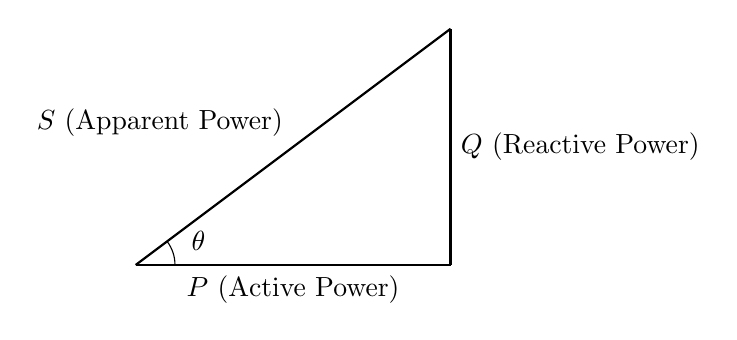
\begin{tikzpicture}
    \draw[thick] (0,0) -- (4,0) node[midway, below] {$P$ (Active Power)};
    \draw[thick] (4,0) -- (4,3) node[midway, right] {$Q$ (Reactive Power)};
    \draw[thick] (0,0) -- (4,3) node[midway, above left] {$S$ (Apparent Power)};
    \draw (0.5,0) arc (0:36.87:0.5);
    \node at (0.8,0.3) {$\theta$};
\end{tikzpicture}
\end{center}

\begin{itemize}
    \item \textbf{Active Power (P)}: Actual power consumed, measured in watts (W), $P = VI \cos\theta$.
    \item \textbf{Reactive Power (Q)}: Power oscillating between source and load, measured in volt-amperes reactive (VAR), $Q = VI \sin\theta$.
    \item \textbf{Power Factor}: Ratio of active power to apparent power, $PF = \cos\theta = P/S$.
\end{itemize}
\end{solutionbox}

\begin{mnemonicbox}
\mnemonic{Real Power Works, Reactive Power Waits}
\end{mnemonicbox}

\questionmarks{2(c) OR}{7}{Explain the structure of atom of trivalent, tetravalent and pentavalent elements.}

\begin{solutionbox}
\begin{center}
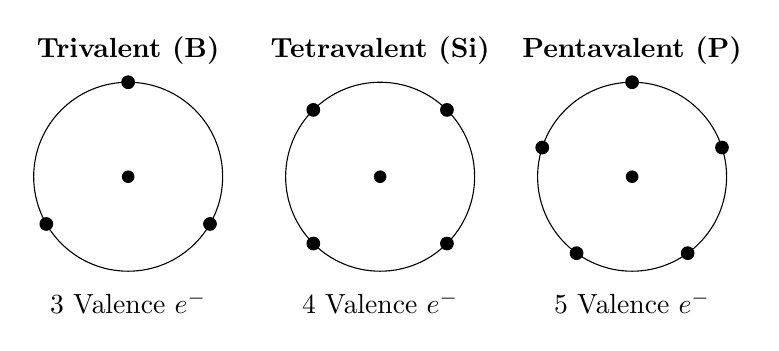
\begin{tikzpicture}[scale=0.8]
    % Trivalent
    \node at (2,4) {\textbf{Trivalent (B)}};
    \draw (2,2) circle (1.5);
    \fill (2,2) circle (0.1);
    \foreach \angle in {90, 210, 330}
        \filldraw (2,2) ++(\angle:1.5) circle (0.1);
    \node at (2,0) {3 Valence $e^-$};

    % Tetravalent
    \node at (6,4) {\textbf{Tetravalent (Si)}};
    \draw (6,2) circle (1.5);
    \fill (6,2) circle (0.1);
    \foreach \angle in {45, 135, 225, 315}
        \filldraw (6,2) ++(\angle:1.5) circle (0.1);
    \node at (6,0) {4 Valence $e^-$};

    % Pentavalent
    \node at (10,4) {\textbf{Pentavalent (P)}};
    \draw (10,2) circle (1.5);
    \fill (10,2) circle (0.1);
    \foreach \angle in {18, 90, 162, 234, 306}
        \filldraw (10,2) ++(\angle:1.5) circle (0.1);
    \node at (10,0) {5 Valence $e^-$};
\end{tikzpicture}
\end{center}

\begin{tabulary}{\linewidth}{|L|L|L|L|}
\hline
\textbf{Element} & \textbf{Structure} & \textbf{Examples} & \textbf{Use} \\ \hline
\textbf{Trivalent} & 3 electrons in outer shell & B, Al, Ga, In & P-type dopant \\ \hline
\textbf{Tetravalent} & 4 electrons in outer shell & Si, Ge, C & Semiconductor base \\ \hline
\textbf{Pentavalent} & 5 electrons in outer shell & P, As, Sb & N-type dopant \\ \hline
\end{tabulary}
\end{solutionbox}

\begin{mnemonicbox}
\mnemonic{Three Accepts, Four Forms, Five Donates}
\end{mnemonicbox}

\questionmarks{3(a)}{3}{Draw the symbol of photodiode and state its application.}

\begin{solutionbox}
\textbf{Symbol:}
\begin{center}
\begin{circuitikz}
    \draw (0,0) to[photodiode] (2,0);
\end{circuitikz}
\captionof{figure}{Photodiode Symbol}
\end{center}

\textbf{Applications:}
\begin{itemize}
    \item Light sensors and detectors.
    \item Optical communication systems.
    \item Solar cells and photovoltaic applications.
    \item Camera exposure controls.
    \item Medical equipment (pulse oximeters).
\end{itemize}
\end{solutionbox}

\begin{mnemonicbox}
\mnemonic{Light Triggers Electric Current}
\end{mnemonicbox}

\questionmarks{3(b)}{4}{Write a Short note on LED.}

\begin{solutionbox}
\textbf{Symbol:}
\begin{center}
\begin{circuitikz}
    \draw (0,0) to[led] (2,0);
\end{circuitikz}
\captionof{figure}{LED Symbol}
\end{center}

\textbf{Information:}
\begin{itemize}
    \item \textbf{Structure}: P-N junction diode that emits light when forward biased.
    \item \textbf{Working Principle}: Electron-hole recombination releases energy as photons.
    \item \textbf{Types}: Various colors based on semiconductor material (GaAs, GaP, GaN).
    \item \textbf{Advantages}: Low power consumption, long life, small size, fast switching.
    \item \textbf{Applications}: Displays, indicators, lighting, remote controls, optical communications.
\end{itemize}
\end{solutionbox}

\begin{mnemonicbox}
\mnemonic{Electrons Jump, Photons Emit}
\end{mnemonicbox}

\questionmarks{3(c)}{7}{Draw and explain VI characteristic of PN junction diode.}

\begin{solutionbox}
\textbf{V-I Characteristics:}
\begin{center}
\begin{tikzpicture}
    \draw[->] (-3,0) -- (3,0) node[right] {$V$};
    \draw[->] (0,-3) -- (0,3) node[above] {$I$};
    \draw[scale=0.5, domain=0:4, smooth, variable=\x, blue, thick] plot ({\x}, {0.05*exp(\x)});
    \draw[scale=0.5, domain=-4:0, smooth, variable=\x, red, thick] plot ({\x}, {-0.1 - 0.1/(1.1+\x)});
    
    \node at (2,2) {Forward Bias};
    \node at (-2,-1) {Reverse Bias};
    \node at (0.7,-0.3) {$V_{k}$};
\end{tikzpicture}
\end{center}

\begin{itemize}
    \item \textbf{Forward Bias Region}:
        \begin{itemize}
            \item Diode conducts when voltage exceeds knee/cut-in voltage (0.3V for Ge, 0.7V for Si).
            \item Current increases exponentially with voltage.
            \item Low resistance state.
        \end{itemize}
    \item \textbf{Reverse Bias Region}:
        \begin{itemize}
            \item Very small leakage current flows.
            \item Current remains almost constant with increasing reverse voltage.
            \item Breakdown occurs at high reverse voltage.
        \end{itemize}
\end{itemize}
\end{solutionbox}

\begin{mnemonicbox}
\mnemonic{Forward Flows Freely, Reverse Resists Rigidly}
\end{mnemonicbox}

\questionmarks{3(a) OR}{3}{List the applications of PN junction diode.}

\begin{solutionbox}
\textbf{Applications:}
\begin{itemize}
    \item Rectification in power supplies.
    \item Signal demodulation.
    \item Logic gates in digital circuits.
    \item Voltage regulation (with zener diodes).
    \item Signal clipping and clamping circuits.
    \item Protection circuits against reverse polarity.
\end{itemize}
\end{solutionbox}

\begin{mnemonicbox}
\mnemonic{Rectify, Detect, Clip, Protect}
\end{mnemonicbox}

\questionmarks{3(b) OR}{4}{Explain the formation of depletion region in unbiased P-N junction.}

\begin{solutionbox}
\textbf{Formation Process:}
\begin{itemize}
    \item Electrons from N-side diffuse into P-side.
    \item Holes from P-side diffuse into N-side.
    \item Recombination occurs at junction.
    \item Immobile ions remain (positive in N-side, negative in P-side).
    \item Electric field develops, opposing further diffusion.
    \item Equilibrium is established, creating depletion region.
\end{itemize}

\begin{center}
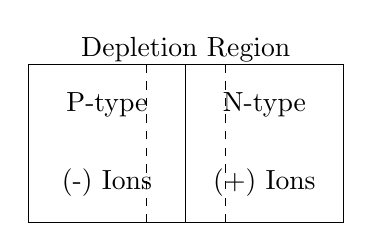
\begin{tikzpicture}
    \draw (0,0) rectangle (4,2);
    \draw (2,0) -- (2,2);
    \node at (1,1.5) {P-type}; \node at (3,1.5) {N-type};
    \node at (1,0.5) {(-) Ions}; \node at (3,0.5) {(+) Ions};
    \draw[dashed] (1.5,0) -- (1.5,2); \draw[dashed] (2.5,0) -- (2.5,2);
    \node at (2,2.2) {Depletion Region};
\end{tikzpicture}
\end{center}
\end{solutionbox}

\begin{mnemonicbox}
\mnemonic{Diffusion Creates Barrier Field}
\end{mnemonicbox}

\questionmarks{3(c) OR}{7}{Explain construction, working and applications of PN junction diode.}

\begin{solutionbox}
\textbf{Construction:}
\begin{itemize}
    \item P-type semiconductor joined with N-type semiconductor.
    \item Made from single crystal of silicon or germanium.
    \item Metal contacts connected to P and N regions.
\end{itemize}

\begin{center}
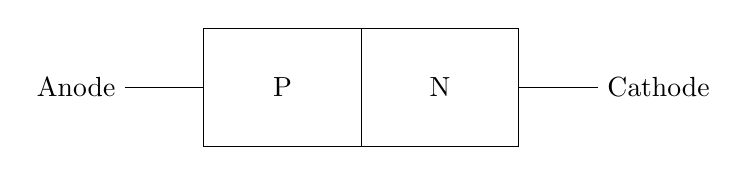
\begin{tikzpicture}
    \draw (0,0) rectangle (4,1.5);
    \draw (2,0) -- (2,1.5);
    \node at (1,0.75) {P}; \node at (3,0.75) {N};
    \draw (0,0.75) -- (-1,0.75) node[left] {Anode};
    \draw (4,0.75) -- (5,0.75) node[right] {Cathode};
\end{tikzpicture}
\end{center}

\textbf{Working:}
\begin{itemize}
    \item \textbf{Forward Bias}: Positive to P, negative to N. Depletion region narrows. Current flows when voltage exceeds barrier potential.
    \item \textbf{Reverse Bias}: Positive to N, negative to P. Depletion region widens. Only small leakage current flows.
\end{itemize}

\textbf{Applications:} Power rectification, Signal detection, Voltage regulation, Switching, Protection circuits.
\end{solutionbox}

\begin{mnemonicbox}
\mnemonic{Join P-N, Control Current Direction}
\end{mnemonicbox}

\questionmarks{4(a)}{3}{Define: (1) Ripple frequency (2) Ripple factor (3) PIV of a diode.}

\begin{solutionbox}
\begin{tabulary}{\linewidth}{|L|L|}
\hline
\textbf{Term} & \textbf{Definition} \\ \hline
\textbf{Ripple Frequency} & Frequency of the AC component remaining in the rectified DC output (2$\times$ input frequency for full-wave, 1$\times$ for half-wave). \\ \hline
\textbf{Ripple Factor} & Ratio of RMS value of AC component to the DC component in rectifier output ($\gamma = V_{ac(rms)}/V_{dc}$). \\ \hline
\textbf{PIV of a diode} & Peak Inverse Voltage is the maximum reverse voltage a diode can withstand without breakdown. \\ \hline
\end{tabulary}
\end{solutionbox}

\begin{mnemonicbox}
\mnemonic{Frequency Fluctuates, Factor Measures, PIV Protects}
\end{mnemonicbox}

\questionmarks{4(b)}{4}{Give comparison between full wave rectifier with two diodes and full wave bridge rectifier.}

\begin{solutionbox}
\begin{tabulary}{\linewidth}{|L|L|L|}
\hline
\textbf{Parameter} & \textbf{Center-Tapped Full Wave} & \textbf{Bridge Rectifier} \\ \hline
\textbf{Number of Diodes} & 2 & 4 \\ \hline
\textbf{Transformer} & Center-tapped required & Simple transformer \\ \hline
\textbf{PIV} & $2V_m$ & $V_m$ \\ \hline
\textbf{Efficiency} & 81.2\% & 81.2\% \\ \hline
\textbf{Ripple Factor} & 0.48 & 0.48 \\ \hline
\textbf{Output} & $V_m/\pi$ & $2V_m/\pi$ \\ \hline
\textbf{Cost} & Higher transformer cost & Higher diode cost \\ \hline
\end{tabulary}
\end{solutionbox}

\begin{mnemonicbox}
\mnemonic{Two Diodes Tap Center, Four Make Bridge}
\end{mnemonicbox}

\questionmarks{4(c)}{7}{Explain zener diode as voltage regulator.}

\begin{solutionbox}
\textbf{Circuit Diagram:}
\begin{center}
\begin{circuitikz}[scale=0.9]
    \draw (0,0) to[sV, l=$V_{in}$] (0,3) to[R, l=$R_S$] (3,3) -- (5,3);
    \draw (3,3) to[zD*, l=$D_Z$] (3,0);
    \draw (5,3) to[R, l=$R_L$] (5,0);
    \draw (0,0) -- (5,0);
    \node at (5.5, 1.5) {$V_{out} = V_Z$};
\end{circuitikz}
\captionof{figure}{Zener Voltage Regulator}
\end{center}

\textbf{Working Principle:}
\begin{itemize}
    \item Zener diode operates in reverse breakdown region.
    \item Maintains constant voltage across its terminals.
    \item Acts as voltage reference.
\end{itemize}

\textbf{Circuit Operation:}
\begin{itemize}
    \item Series resistor $R_S$ limits current.
    \item Zener conducts when input exceeds breakdown voltage.
    \item Excess current flows through zener diode.
    \item Output voltage remains constant at zener voltage.
\end{itemize}

\textbf{Advantages:} Simple circuit, Low cost, Good regulation for small load changes.
\end{solutionbox}

\begin{mnemonicbox}
\mnemonic{Zener Breaks Down to Hold Voltage Steady}
\end{mnemonicbox}

\questionmarks{4(a) OR}{3}{What is rectifier? Explain full wave rectifier with waveforms.}

\begin{solutionbox}
\textbf{Rectifier:} A circuit that converts AC voltage to pulsating DC voltage.

\textbf{Full Wave Rectifier (Center-Tapped):}
\begin{center}
\begin{circuitikz}[scale=0.8]
    \draw (0,0) node[transformer core] (T) {};
    \draw (T.A1) -- ++(-0.5,0) node[left] {AC};
    \draw (T.A2) -- ++(-0.5,0);
    \draw (T.B1) to[D*, l=$D_1$] (3,1);
    \draw (T.B2) to[D*, l=$D_2$] (3,-1);
    \draw (3,1) -- (3,-1);
    \draw (3,0) to[R, l=$R_L$] (5,0);
    \draw (T.base) -- (5,0) |- (5,0);
\end{circuitikz}
\end{center}

\textbf{Waveforms:}
\begin{center}
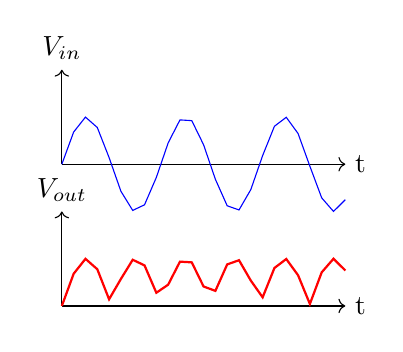
\begin{tikzpicture}[scale=0.6]
    % Input
    \draw[->] (0,3) -- (6,3) node[right] {t};
    \draw[->] (0,3) -- (0,5) node[above] {$V_{in}$};
    \draw[blue] plot[domain=0:6] (\x, {3 + sin(\x r * 3)});
    
    % Output
    \draw[->] (0,0) -- (6,0) node[right] {t};
    \draw[->] (0,0) -- (0,2) node[above] {$V_{out}$};
    \draw[red, thick] plot[domain=0:6] (\x, {abs(sin(\x r * 3))});
\end{tikzpicture}
\captionof{figure}{Full Wave Rectifier Waveforms}
\end{center}
\end{solutionbox}

\begin{mnemonicbox}
\mnemonic{Both Half-Cycles Become Positive}
\end{mnemonicbox}

\questionmarks{4(b) OR}{4}{Why filter is required in rectifier? State the different types of filter and explain any one type of filter.}

\begin{solutionbox}
\textbf{Need for Filter:}
\begin{itemize}
    \item Rectifier output contains AC ripple component.
    \item Pure DC required for electronic circuits.
    \item Filters smooth pulsating DC by removing AC components.
\end{itemize}

\textbf{Types of Filters:} Capacitor (C), Inductor (L), LC, $\pi$ (Pi), CLC filter.

\textbf{Capacitor Filter:}
\begin{center}
\begin{circuitikz}
    \draw (0,0) to[short, o-o] (0,2);
    \draw (0,2) -- (2,2) to[C, l=C] (2,0) -- (0,0);
    \draw (2,2) -- (4,2) to[R, l=$R_L$] (4,0) -- (2,0);
    \node at (-0.5,1) {Rectifier Out};
    \node at (5,1) {DC Out};
\end{circuitikz}
\captionof{figure}{Capacitor Filter}
\end{center}

\textbf{Working:}
\begin{itemize}
    \item Capacitor charges during voltage rise.
    \item Discharges slowly during voltage fall.
    \item Reduces ripple voltage.
\end{itemize}
\end{solutionbox}

\begin{mnemonicbox}
\mnemonic{Capacitor Catches Peaks, Releases Slowly}
\end{mnemonicbox}

\questionmarks{4(c) OR}{7}{Write the need of rectifier. Explain bridge rectifier with circuit diagram and draw its input and output waveforms.}

\begin{solutionbox}
\textbf{Need of Rectifier:} Convert AC to DC for electronic devices, power supplies, charging systems.

\textbf{Bridge Rectifier Circuit:}
\begin{center}
\begin{circuitikz}[scale=0.8]
    \draw (0,0) to[sV, l=$V_{in}$] (0,3);
    \draw (0,3) -- (2,3) -- (3,2);
    \draw (0,0) -- (2,0) -- (5,0) -- (5,2);
    
    % Bridge
    \draw (3,2) to[D*, l=$D_1$] (4,3);
    \draw (4,3) to[D*, l=$D_2$] (5,2);
    \draw (5,2) to[D*, l=$D_3$] (4,1);
    \draw (4,1) to[D*, l=$D_4$] (3,2);
    
    % Load
    \draw (4,3) -- (4,4) -- (7,4) to[R, l=$R_L$] (7,0) -- (5,0);
    \draw (4,1) -- (4,0);
\end{circuitikz}
\captionof{figure}{Bridge Rectifier}
\end{center}

\textbf{Waveforms:} Input is sine wave, Output is pulsating DC (full-wave rectified).
\end{solutionbox}

\begin{mnemonicbox}
\mnemonic{Four Diodes Direct All Current One Way}
\end{mnemonicbox}

\questionmarks{5(a)}{3}{Explain causes of electronic waste.}

\begin{solutionbox}
\textbf{Causes:}
\begin{itemize}
    \item Rapid technological advancement.
    \item Planned obsolescence of products.
    \item Decreasing product lifespan.
    \item Consumer behavior preferring new devices.
    \item Limited repair options for electronics.
    \item High repair costs compared to replacement.
\end{itemize}
\end{solutionbox}

\begin{mnemonicbox}
\mnemonic{Technology Advances, Products Expire Rapidly}
\end{mnemonicbox}

\questionmarks{5(b)}{4}{Compare PNP and NPN transistors.}

\begin{solutionbox}
\begin{tabulary}{\linewidth}{|L|L|L|}
\hline
\textbf{Parameter} & \textbf{PNP Transistor} & \textbf{NPN Transistor} \\ \hline
\textbf{Symbol} & \begin{circuitikz}[scale=0.6]\draw(0,0)node[pnp]{};\end{circuitikz} & \begin{circuitikz}[scale=0.6]\draw(0,0)node[npn]{};\end{circuitikz} \\ \hline
\textbf{Majority Carriers} & Holes & Electrons \\ \hline
\textbf{Current Flow} & Emitter to Collector & Collector to Emitter \\ \hline
\textbf{Biasing} & Emitter +ve, Base -ve & Collector +ve, Base +ve \\ \hline
\textbf{Switching Speed} & Slower & Faster \\ \hline
\end{tabulary}
\end{solutionbox}

\begin{mnemonicbox}
\mnemonic{Negative-Positive-Negative vs Positive-Negative-Positive}
\end{mnemonicbox}

\questionmarks{5(c)}{7}{Draw the symbol, explain the construction and working of MOSFET.}

\begin{solutionbox}
\textbf{Symbol:}
\begin{center}
\begin{circuitikz}
    \draw (0,0) node[nmos] (Q) {};
    \node[right] at (Q.D) {D};
    \node[right] at (Q.S) {S};
    \node[left] at (Q.G) {G};
\end{circuitikz}
\captionof{figure}{MOSFET Symbol}
\end{center}

\textbf{Construction:}
\begin{center}
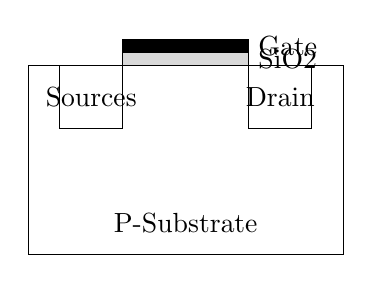
\begin{tikzpicture}[scale=0.8]
    \draw (0,0) rectangle (5,3);
    \node at (2.5,0.5) {P-Substrate};
    \draw[fill=white] (0.5,2) rectangle (1.5,3); \node at (1,2.5) {Sources};
    \draw[fill=white] (3.5,2) rectangle (4.5,3); \node at (4,2.5) {Drain};
    \draw[fill=gray!30] (1.5,3) rectangle (3.5,3.2); \node[right] at (3.5,3.1) {SiO2};
    \draw[fill=black] (1.5,3.2) rectangle (3.5,3.4); \node[right] at (3.5,3.3) {Gate};
\end{tikzpicture}
\captionof{figure}{MOSFET Construction}
\end{center}

\textbf{Working Principle (Enhancement Mode):}
\begin{itemize}
    \item No channel exists without gate voltage.
    \item Positive gate voltage attracts electrons from substrate.
    \item Induced channel allows current flow from drain to source.
    \item Increasing gate voltage enhances conductivity.
\end{itemize}
\end{solutionbox}

\begin{mnemonicbox}
\mnemonic{Gate Voltage Creates Electron Channel}
\end{mnemonicbox}

\questionmarks{5(a) OR}{3}{Explain methods to handle electronic waste.}

\begin{solutionbox}
\textbf{Methods:}
\begin{tabulary}{\linewidth}{|L|L|}
\hline
\textbf{Method} & \textbf{Description} \\ \hline
\textbf{Reduce} & Designing longer-lasting electronics. \\ \hline
\textbf{Reuse} & Donating or selling functional devices. \\ \hline
\textbf{Recycle} & Material recovery (precious metals). \\ \hline
\textbf{Regulation} & E-waste management policies. \\ \hline
\textbf{Recovery} & Extracting valuable materials. \\ \hline
\end{tabulary}
\end{solutionbox}

\begin{mnemonicbox}
\mnemonic{Reduce, Reuse, Recycle, Regulate, Recover}
\end{mnemonicbox}

\questionmarks{5(b) OR}{4}{Derive the relationship between $\alpha_{dc}$ and $\beta_{dc}$.}

\begin{solutionbox}
\textbf{Relations:} $I_E = I_C + I_B$, $\alpha_{dc} = I_C/I_E$, $\beta_{dc} = I_C/I_B$.

\textbf{Derivation:}
\begin{itemize}
    \item From $I_E = I_C + I_B$, divide by $I_C$:
    $$ \frac{I_E}{I_C} = 1 + \frac{I_B}{I_C} $$
    $$ \frac{1}{\alpha_{dc}} = 1 + \frac{1}{\beta_{dc}} $$
    $$ \frac{1}{\alpha_{dc}} = \frac{\beta_{dc} + 1}{\beta_{dc}} $$
    $$ \alpha_{dc} = \frac{\beta_{dc}}{1+\beta_{dc}} $$
    \item Rearranging for $\beta_{dc}$:
    $$ \beta_{dc} = \frac{\alpha_{dc}}{1-\alpha_{dc}} $$
\end{itemize}
\end{solutionbox}

\begin{mnemonicbox}
\mnemonic{Alpha-Beta Relate as Alpha = Beta/(1+Beta)}
\end{mnemonicbox}

\questionmarks{5(c) OR}{7}{Explain common collector configuration with its input and output characteristics.}

\begin{solutionbox}
\textbf{Common Collector (Emitter Follower):}
\begin{center}
\begin{circuitikz}
    \draw (0,0) node[npn] (Q) {};
    \draw (Q.C) -- ++(0,1) node[above] {$V_{CC}$};
    \draw (Q.B) to[R, l=$R_B$] (-2,0) to[sV, l=$V_{in}$] (-2,-2) -- (0,-2) -- (Q.E);
    \draw (Q.E) to[R, l=$R_E$] (0,-2) node[ground] {};
    \draw (Q.E) -- ++(2,0) to[short, -o] ++(0,0) node[right] {$V_{out}$};
\end{circuitikz}
\captionof{figure}{Common Collector Circuit}
\end{center}

\textbf{Characteristics:}
\begin{itemize}
    \item \textbf{Input Characteristics}: Plot of $I_B$ vs $V_{BC}$. High input impedance.
    \item \textbf{Output Characteristics}: Plot of $I_E$ vs $V_{CE}$. Low output impedance.
\end{itemize}

\textbf{Key Features:} Voltage gain $\approx 1$, High current gain ($\beta+1$), used as buffer.
\end{solutionbox}

\begin{mnemonicbox}
\mnemonic{Emitter Follows Base Voltage}
\end{mnemonicbox}

\end{document}
